\documentclass[a4paper]{article}
\usepackage[spanish, es-lcroman]{babel}   % es-lcroman: for roman in lower-case in enumerate
\usepackage{graphicx}
\pagestyle{headings}
\titlepage
\usepackage[utf8]{inputenc} 		% para codificacion unicode (utf8)
\usepackage{enumerate}
\usepackage{hyperref}			% para links a paginas web
\usepackage{subfig}
\usepackage{graphics}
\usepackage{amsmath}
\usepackage{amssymb}
\usepackage{amsthm}
\usepackage{placeins}
%\usepackage{tabularx}
\usepackage{booktabs,siunitx}
%\usepackage{fullpage}

\decimalpoint

% That follow if for listings configuration
\usepackage{listings}
\usepackage{color}
\usepackage{textcomp}
\definecolor{listinggray}{gray}{0.9}
\definecolor{lbcolor}{rgb}{0.99,0.99,0.99}
\lstset{
    backgroundcolor=\color{lbcolor},
    tabsize=4,
    rulecolor=,
    language=matlab,
        basicstyle=\scriptsize,
        upquote=true,
        aboveskip={1.5\baselineskip},
        columns=fixed,
        showstringspaces=false,
        extendedchars=true,
        breaklines=true,
        prebreak = \raisebox{0ex}[0ex][0ex]{\ensuremath{\hookleftarrow}},
        frame=single,
        showtabs=false,
        showspaces=false,
        showstringspaces=false,
        identifierstyle=\ttfamily,
        keywordstyle=\color[rgb]{0,0,1},
        commentstyle=\color[rgb]{0.133,0.545,0.133},
        stringstyle=\color[rgb]{0.627,0.126,0.941},
}

\newcommand{\X}{\mathbf{X}}
\newcommand{\V}{\mathbf{V}}
\newcommand{\W}{\mathbf{W}}
\newcommand{\Hbf}{\mathbf{H}}
\newcommand{\vbf}{\mathbf{v}}
\newcommand{\h}{\mathbf{h}}
\newcommand{\A}{\mathbf{A}}
\newcommand{\B}{\mathbf{B}}
\newcommand{\x}{\mathbf{x}}

\DeclareMathOperator*{\argmin}{arg\,min}
\DeclareMathOperator*{\argmax}{arg\,max}

\newtheorem*{theorem*}{Teorema}

\title{Definiciones de potencia y densidad espectral de potencia de señales en tiempo continuo}
\author{Ernesto López}

\begin{document} 

\maketitle

\section{Introducción}

En este documento se presentan los conceptos de energía, potencia y densidades espectrales de señales en tiempo continuo. Se diferencian los casos de señales determinísticas y procesos aleatorios. Se clasifican las señales en señales de energía y señales de potencia y se incluye el teorema de Wiener-Khintchine, el cual demuestra que la función de autocorrelación y la densidad espectral de potencia de señales aleatorias forman un par de transformadas de Fourier. Finalmente, se incluye la deducción de la densidad espectral de potencia de una señal modulada por amplitud de pulsos (PAM, \emph{Pulse Amplitude Modulation}) digital.

Lo incluido en este documento constituye una parte de un tema de un curso sobre sistemas de comunicación. Todo lo aquí presentado está basado en los capítulos 2, 3 y 9 del libro \cite{lathi1990modern4th}.

\section{Señales determinísticas}

\subsection{Energía y potencia de una señal}\label{sec:signal_energy_and_power_definition}

Desde un punto de vista cualitativo, la energía y la potencia de una señal son medidas del \emph{tamaño} de la señal.
La \textbf{energía} \(E_g\) de una señal \(g(t)\) se define como el área bajo la curva \(g^2(t)\),
\begin{equation}\label{eq:signal_energy_definition}
 E_g = \int_{-\infty}^{\infty}g^2(t)\,dt. 
\end{equation}
Esta definición es válida para señales reales. Si la señal toma valores complejos, la definición se generaliza a
\[
 E_g = \int_{-\infty}^{\infty}|g(t)|^2\,dt.
\]
Algunas observaciones respecto a la definición son las siguientes:
\begin{itemize}
 \item El área bajo \(g(t)\) no sería apropiada como medida del tamaño de la señal, ya que el área de las partes positivas se cancela con el área de las partes negativas de \(g(t)\). Si bien se podría haber elegido otra definición, como por ejemplo, la integral de \(|g(t)|\), la definición dada por la ecuación \ref{eq:signal_energy_definition} es matemáticamente mas tratable. 
 \item La energía de una señal puede ser infinita. Esto ocurre si la integral de la ecuación \ref{eq:signal_energy_definition} no converge.  Una condición necesaria para que una señal \(g(t)\) tenga energía finita es que \(\lim_{|t|\to\infty}g(t)=0\). Las señales periódicas son un ejemplo de señales con energía infinita.
\end{itemize}

La energía de una señal es significativa como medida de tamaño si es finita. En caso contrario, una medida mas significativa es la \textbf{potencia}, definida como el promedio temporal de la energía,
\begin{equation}\label{eq:signal_power_definition}
 P_g =  \lim_{T\to\infty}\frac{1}{T}\int_{-T/2}^{T/2}g^2(t)\,dt.
\end{equation}
Esta expresión es válida si \(g(t)\) es real. La generalización para señales complejas es análoga a la generalización de la definición de la energía. Conviene hacer algunas observaciones sobre esta definición:
\begin{itemize}
 \item La potencia es el promedio temporal de la amplitud al cuadrado de la señal \(g(t)\), es decir, el \textbf{valor cuadrático medio} de \(g(t)\). La raíz cuadrada de la potencia es el valor \textbf{rms} (root-mean square) de \(g(t)\).
 \item Como la potencia es el valor cuadrático medio de \(g(t)\) y \(g(t)\) toma en general valores finitos, la potencia es \textbf{finita}. Ejemplos de señales de potencia infinita, son aquellas que cumplen que \(\lim_{|t|\to\infty}g(t)=\pm\infty\), como la señal \(g(t)=t\).
\end{itemize}

En este contexto, los conceptos de energía y potencia son características intrínsecas de señales que proveen información sobre el \emph{tamaño} de la señal y no son los mismos que las nociones de energía y potencia en física. Por ejemplo, una medida apropiada de la similitud entre dos señales \(g(t)\) y \(z(t)\), es la potencia de la señal diferencia \(e(t)=g(t)-z(t)\), magnitud conocida como el \textbf{error cuadrático medio} entre \(g(t)\) y \(z(t)\). Otro ejemplo importante de aplicación es en la medición de la \textbf{relación señal a ruido}, magnitud definida como el cociente de la potencia de cierta señal deseada y la potencia de cierta señal contaminante.

Las unidades estándar de energía y potencia son respectivamente el Joule (J) y el Watt (W). Sin embargo, al referirse a señales, los conceptos de energía y potencia no están vinculados a las magnitudes físicas, y las unidades dependen de las unidades de la señal \(g(t)\). Si \(g(t)\) tiene unidades de voltaje (V), las unidades de la energía \(E_g\) son voltios al cuadrado segundos (\(\textrm{V}^2\)s) y las de la potencia \(P_g\) son voltios al cuadrado  (\(\textrm{V}^2\)). Si \(g(t)\) es intensidad eléctrica, las unidades son amperes al cuadrado segundos (\(\textrm{A}^2\)s) y amperes al cuadrado (\(\textrm{A}^2\)) respectivamente. Es común en la bibliografía, asumir que \(g(t)\) es una señal de voltaje aplicada a una carga de resistencia 1 ohm (\(\Omega\)). En ese caso, la energía \(E_g\) coincide con la energía disipada por la resistencia, y las unidades son Jules (\(\textrm{V}^2\textrm{s}/\Omega\)). La misma idea se aplica a la potencia \(P_g\), que se interpreta como la potencia promedio consumida por la resistencia, con unidades de Watts (J/s o \(\textrm{V}^2/\Omega\)).

\subsection{Señales de energía y de potencia}

Se llama \textbf{señal de energía} a una señal que tiene energía finita. Concretamente, la señal \(g(t)\) es de energía si cumple que
\[
 \int_{-\infty}^{\infty}|g(t)|^2\,dt < \infty.
\]
De forma similar, una señal con potencia no nula y finita se llama \textbf{señal de potencia}. Es decir, una señal \(g(t)\) es de potencia si cumple que
\[
 0 < \lim_{T\to\infty}\frac{1}{T}\int_{-T/2}^{T/2}|g(t)|^2\,dt < \infty.
\]
Observaciones:
\begin{itemize}
  \item Como la potencia es el promedio temporal de la energía en un intervalo infinitamente largo, una señal con energía finita (señal de energía) tiene potencia nula. Por la misma razón, una señal con potencia finita (señal de potencia), tiene energía infinita. Se concluye que una señal no puede ser simultáneamente de energía y de potencia. Señales con potencia infinita, como \(g(t)=t\), no son de energía ni de potencia.
  \item Una señal de soporte temporal finito, es de energía. Las señales de soporte temporal infinito, como por ejemplo, las señales periódicas, son de potencia.
  \item Las señales realizables en la práctica, siempre tienen soporte temporal acotado y toman valores finitos en ese soporte. Por lo tanto, las señales realizables son siempre de energía. Es imposible generar señales de potencia en la práctica, porque requieren duración y energía infinita.
\end{itemize}

\subsection{Densidad Espectral de Energía}

\subsubsection{Cálculo de la energía en el dominio de la frecuencia}

La energía de una señal \(g(t)\) se definió como el área bajo \(|g(t)|^2\) (ecuación \ref{eq:signal_energy_definition} para \(g(t)\) real). Mediante el teorema de Parseval, también es posible calcular la energía en el dominio de la frecuencia mediante la transformada de Fourier\footnote{Recurrir al apéndice \ref{ap:fourier_transform} por una breve introducción a la transformada de Fourier.} \(G(f)\) de \(g(t)\) como 
\begin{equation}\label{eq:signal_energy_freq_domain}
 E_g = \int_{-\infty}^{\infty}|G(f)|^2\,df.
\end{equation}
Para demostrarlo, se parte de la definición de la energía y se opera de la siguiente forma,
\begin{align*}
 E_g &= \int_{-\infty}^{\infty}g(t)g^*(t)\,dt\\
  &\overset{(a)}{=}\int_{-\infty}^{\infty}g(t)\left[\int_{-\infty}^{\infty}G^*(f)e^{-j2\pi ft}\,df\right]\,dt\\
  &\overset{(b)}{=}\int_{-\infty}^{\infty}G^*(f)\left[\int_{-\infty}^{\infty}g(t)e^{-j2\pi ft}\,dt\right]\,df\\
  &\overset{(c)}{=}\int_{-\infty}^{\infty}G(f)G^*(f)\,df\\
  &=\int_{-\infty}^{\infty}|G(f)|^2\,df,
\end{align*}
donde en \((a)\) se usó la antitransformada de Fourier (ecuación \ref{eq:inverse_fourier_transform_def}) conjugada, en \((b)\) se cambió el orden de integración y en \((c)\) se reconoce que el término entre paréntesis rectos es la transformada de Fourier de \(g(t)\) (ecuación \ref{eq:fourier_transform_def}). El cambio del orden de integración realizado en \((b)\) puede hacerse debido a que se asume que se trata de una señal de energía, y como la energía es finita, las integrales convergen.

\subsubsection{Densidad Espectral de Energía}

La ecuación \ref{eq:signal_energy_freq_domain} puede interpretarse como que la energía total de la señal \(g(t)\) es resultado de la energía contribuida por cada componente espectral de \(g(t)\). La contribución del componente espectral de frecuencia \(f\) es proporcional a \(|G(f)|^2\). Esta interpretación motiva la definición de la \textbf{Densidad Espectral de Energía} (ESD, \emph{Energy Spectral Density}) \(\Psi_g(f)\) como
\[
 \Psi_g(f) = |G(f)|^2.
\]
De esta forma, la energía total de la señal \(g(t)\) se calcula como la integral de la Densidad Espectral de Energía en todas las frecuencias,
\[
 E_g = \int_{-\infty}^{\infty}\Psi_g(f)\,df,
\]
acorde con la ecuación \ref{eq:signal_energy_freq_domain}.

\subsubsection{Función de autocorrelación}\label{sec:energy_signal_autocorr}

La función de autocorrelación es una medida de similitud de una señal consigo misma. Su importancia radica en que provee información valiosa sobre el contenido espectral de la señal. La función de autocorrelación \(\psi_g(\tau)\) de una señal \(g(t)\) real determinística se define como,
\begin{equation}\label{eq:deterministic_autocorr_def}
 \psi_g(\tau)=\int_{-\infty}^{\infty}g(t)g(t+\tau)\,dt.
\end{equation}
En el caso de una señal \(g(t)\) determinística que toma valores complejos, la función de autocorrelación se define como,
\[
 \psi_g(\tau)=\int_{-\infty}^{\infty}g(t)g^*(t-\tau)\,dt = \int_{-\infty}^{\infty}g^*(t)g(t+\tau)\,dt.
\]

Una propiedad importante de la función de autocorrelación es que es una función \textbf{simétrica conjugada}, es decir, se cumple que \(\psi_g(-\tau)=\psi_g^*(\tau)\). Para ver esto, se parte de la definición de la función de autocorrelación evaluada en \(-\tau\), \(\psi_g(-\tau)\), y se opera de la siguiente forma
\begin{align*}
 \psi_g(-\tau) &= \int_{-\infty}^{\infty}g^*(t)g(t-\tau)\,dt\\
  &\overset{(a)}{=}\int_{-\infty}^{\infty}g^*(x+\tau)g(x)\,dx\\
  &\overset{(b)}{=}\left[\int_{-\infty}^{\infty}g^*(x)g(x+\tau)\,dx\right]^*\\
  &\overset{(c)}{=}\psi_g^*(\tau),
\end{align*}
donde en \((a)\) se realizó el cambio de variable \(x=t-\tau\), en \((b)\) se conjugó la integral y su argumento, y en \((c)\) se reconoce que la expresión entre paréntesis rectos es \(\psi_g(\tau)\). En el caso particular en que \(g(t)\) es real, la autocorrelación es real, y además, esta propiedad indica que es una función \textbf{par}, es decir, se cumple que \(\psi_g(\tau)=\psi_g(-\tau)\).

\subsubsection{Relación entre la función de autocorrelación y la ESD}\label{sec:autocorr_and_esd_relation}

La función de autocorrelación \(\psi_g(\tau)\) y la ESD \(\Psi_g(f)\) de una señal \(g(t)\) forman un par de transformadas de Fourier,
\[
\psi_g(\tau)\overset{\mathcal{F}}{\longleftrightarrow}\Psi_g(f).
\]
Demostración: se probará el caso mas general de \(g(t)\) compleja. Se parte de la transformada de Fourier de la autocorrelación \(\psi_g(\tau)\) y se opera de la siguiente forma,
\begin{align*}
 \mathcal{F}\left[\psi_g(\tau)\right] &\overset{(a)}{=} \int_{-\infty}^{\infty}\psi_g(\tau)e^{-j2\pi f\tau}\,d\tau\\
  &\overset{(b)}{=}\int_{-\infty}^{\infty}\left[\int_{-\infty}^{\infty}g^*(t)g(t+\tau)\,dt\right]e^{-j2\pi f\tau}\,d\tau\\
  &\overset{(c)}{=}\int_{-\infty}^{\infty}g^*(t)\left[\int_{-\infty}^{\infty}g(t+\tau)e^{-j2\pi f\tau}\,d\tau\right]\,dt,
\end{align*}
donde en \((a)\) se aplicó la definición de la transformada de Fourier (ecuación \ref{eq:fourier_transform_def}) reconociendo que la variable independiente de la autocorrelación es \(\tau\), en \((b)\) se sustituyó la definición de la autocorrelación \(\psi_g(\tau)\) de una señal \(g(t)\) compleja y en \((c)\) se cambió el orden de integración. La expresión entre paréntesis rectos en la última igualdad es la transformada de Fourier de \(g(\tau+t)\), que no es otra cosa que la función \(g(\tau)\) desplazada una cantidad \(t\) hacia la izquierda. Usando la propiedad de desplazamiento temporal de la transformada de Fourier (ver apéndice \ref{ap:fourier_transform_property_time_shift}), se tiene que
\[
 \mathcal{F}\left[g(\tau+t)\right] = e^{j2\pi ft}G(f),
\]
y empleando este resultado en el razonamiento, se llega a que
\begin{align*}
 \mathcal{F}\left[\psi_g(\tau)\right] & = G(f)\int_{-\infty}^{\infty}g^*(t)e^{j2\pi ft}\,dt,\\ 
  &\overset{(b)}{=}G(f)G^*(f)\\
  & = |G(f)|^2,
\end{align*}
donde en la igualdad \((b)\) se reconoce que la integral es la transformada de Fourier conjugada de \(g(t)\). Se concluye que
\[
 \psi_g(\tau)\quad\overset{\mathcal{F}}{\longleftrightarrow}\quad\Psi_g(f)=|G(f)|^2,
\]
o explícitamente,
\[
 \int_{-\infty}^{\infty}g^*(t)g(t+\tau)\,dt\quad\overset{\mathcal{F}}{\longleftrightarrow}\quad|G(f)|^2,
\]
donde \(G(f)=\mathcal{F}\left[g(t)\right]\) y \(g(t)\) es una señal de energía.

Notar que la ESD, por ser el módulo al cuadrado de una función compleja, es siempre una función \textbf{real y positiva}. Adicionalmente, si \(g(t)\) es real, la ESD es, además de real y positiva, \textbf{par}. Esto se debe a que la autocorrelación de una señal real es una función real y par, y por lo tanto, su transformada de Fourier también es real y par.  En el apéndice \ref{ap:fourier_transform_property_symmetry} se demuestra esta propiedad de la transformada de Fourier.

\subsection{Densidad Espectral de Potencia}

\subsubsection{Relación entre la potencia y la energía}

En el caso de señales de potencia, la magnitud apropiada como medida de tamaño de una señal es la potencia. La potencia de una señal fue definida en la sección \ref{sec:signal_energy_and_power_definition} y está dada por la ecuación \ref{eq:signal_power_definition},
\[
 P_g =  \lim_{T\to\infty}\frac{1}{T}\int_{-T/2}^{T/2}g^2(t)\,dt.
\]
Con el objetivo de vincular los conceptos de energía y potencia así como definir la Densidad Espectral de Potencia, se considera a la señal \(g(t)\) truncada en el tiempo de la siguiente forma,
\begin{equation}\label{eq:temporal_truncated_g}
 g_T(t)=
  \left\{\begin{array}{ll}
  g(t) & |t| \leq T/2\\
  0 & |t| > T/2\\ \end{array} \right..
\end{equation}
 Por ser de soporte finito, la señal \(g_T(t)\) es una señal de energía, con la energía dada por
 \[
  E_{g_T}=\int_{-\infty}^{\infty}g_T^2(t)\,dt=\int_{-T/2}^{T/2}g_T^2(t)\,dt=\int_{-T/2}^{T/2}g^2(t)\,dt.
 \]
 Sustituyendo este resultado en la ecuación de la potencia, se obtiene la relación entre la energía y la potencia,
 \[
  P_g =  \lim_{T\to\infty}\frac{E_{g_T}}{T},
 \]
indicando que la potencia es el promedio temporal de la energía.
 
\subsubsection{Densidad Espectral de Potencia}\label{sec:psd_deterministic}
 
El teorema de Parseval (ecuación \ref{eq:signal_energy_freq_domain}) indica que la energía de \(g_T(t)\) puede determinarse en el dominio de la frecuencia como
\[
 E_{g_T}=\int_{-\infty}^{\infty}|G_T(f)|^2\,df,
\]
donde \(G_T(f)\) es la transformada de Fourier de la señal truncada, \(G_T(f)=\mathcal{F}\left[g_T(t)\right]\). Por lo tanto, la potencia de \(g(t)\) se puede calcular como
\begin{equation}\label{eq:psd_derivation_tmp}
 P_g =  \lim_{T\to\infty}\frac{E_{g_T}}{T} = \lim_{T\to\infty}\frac{1}{T}\int_{-\infty}^{\infty}|G_T(f)|^2\,df.
\end{equation}
Como \(g(t)\) es una señal de potencia, su energía es infinita. La señal truncada \(g_T(t)\) es de energía, y por lo tanto, su energía \(E_{g_T}\) es finita si \(T\) es finito, pero tiende a infinito con \(T\). Esto implica que \(|G_T(f)|^2\) también tiende a infinito con \(T\). Sin embargo, la velocidad de crecimiento de \(|G_T(f)|^2\) debe ser igual a \(T\) para que la potencia sea finita, por tratarse de una señal de potencia, y la expresión de la izquierda en la ecuación \ref{eq:psd_derivation_tmp} converja. Esta convergencia permite intercambiar el orden del límite y la integración en la ecuación \ref{eq:psd_derivation_tmp}, resultando en
\begin{equation}\label{eq:signal_power_freq_domain}
 P_g = \int_{-\infty}^{\infty}\lim_{T\to\infty}\frac{|G_T(f)|^2}{T}\,df.
\end{equation}
Esta expresión motiva la definición de la \textbf{Densidad Espectral de Potencia} (PSD, \emph{Power Spectral Density}) como,
\begin{equation}\label{eq:psd_definition}
 S_g(f) = \lim_{T\to\infty}\frac{|G_T(f)|^2}{T},
\end{equation}
ya que de esta forma, la potencia es la integral de la Densidad Espectral de Potencia en todas las frecuencias, es decir,
\[
 P_g = \int_{-\infty}^{\infty}S_g(f)\,df.
\]

Al igual que la ESD, la PSD es una función \textbf{positiva} y \textbf{real}, y si \(g(t)\) es real, también es \textbf{par}. Si \(g(t)\) es una señal de voltaje, la PSD tiene unidades de volitos al cuadrado por Hertz (\(\textrm{V}^2/\textrm{Hz}\)).

\subsubsection{Función de autocorrelación de señales de potencia}

La función de autocorrelación de una señal de potencia \(g(t)\) real se define como
\begin{equation}\label{eq:deterministic_autocorr_power_signal_def}
 \mathcal{R}_g(\tau)=\lim_{T\to\infty}\frac{1}{T}\int_{-T/2}^{T/2}g(t)g(t+\tau)\,dt.
\end{equation}
La extensión al caso complejo es análoga a la función de autocorrelación de una señal de energía (ver sección \ref{sec:energy_signal_autocorr}). Es una función \textbf{simétrica conjugada},
\[
 \mathcal{R}_g(-\tau) = \mathcal{R}^*_g(\tau),
\]
o \textbf{par} si \(g(t)\) es real.

Notar que la autocorrelación \(\mathcal{R}_g(\tau)\) es el promedio temporal de \(g(t)g(t+\tau)\),
\[
 \mathcal{R}_g(\tau) = \left<g(t)g(t+\tau)\right>.
\]
Es importante resaltar que se trata de la \textbf{media temporal} y no de la media estadística, ya que la señal \(g(t)\) se consideró determinística en todo lo discutido hasta ahora. Por lo tanto, la terminología apropiada para la autocorrelación definida por la ecuación \ref{eq:deterministic_autocorr_power_signal_def} debería ser \textbf{autocorrelación temporal} o \textbf{autocorrelación determinística}. En contraposición, la autocorrelación de un proceso aleatorio \(g(t)\) se define como la media estadística de  \(g(t)g(t+\tau)\), denotada como   \(\overline{g(t)g(t+\tau)}\) o \(E\{g(t)g(t+\tau)\}\). Los conceptos análogos para el caso de procesos aleatorios se tratan mas adelante.

\subsubsection{Relación entre la función de autocorrelación y la PSD}\label{sec:autocorr_and_psd_relation}

Análogamente a lo que ocurre con las señales de energía, la autocorrelación y la PSD de una señal de potencia forman un par de transformadas de Fourier,
\[
 \mathcal{R}_g(\tau)\overset{\mathcal{F}}{\longleftrightarrow}S_g(f).
\]
Para ver esto, se considera la señal trucada \(g_T(t)\) definida en la ecuación \ref{eq:temporal_truncated_g}. \(g_T(t)\) es una señal de energía con autocorrelación y ESD \(\psi_{g_T}(\tau)\) y \(\Psi_{g_T}(f)\) respectivamente, y por lo tanto, se cumple que
\[
 \psi_{g_T}(\tau)\overset{\mathcal{F}}{\longleftrightarrow}\Psi_{g_T}(f)=|G_T(f)|^2,
\]
como se explicó en la sección \ref{sec:autocorr_and_esd_relation}. Considerando a la señal truncada, la autocorrelación de la ecuación \ref{eq:deterministic_autocorr_power_signal_def} puede escribirse como
\[
 \mathcal{R}_g(\tau)=\lim_{T\to\infty}\frac{1}{T}\int_{-T/2}^{T/2}g_T(t)g_T(t+\tau)\,dt=\lim_{T\to\infty}\frac{\psi_{g_T}(\tau)}{T}.
\]
Aplicando la transformada de Fourier, se tiene que
\[
  \mathcal{F}\left[\mathcal{R}_g(\tau)\right]=\lim_{T\to\infty}\frac{\Psi_{g_T}(f)}{T}=\lim_{T\to\infty}\frac{|G_T(f)|^2}{T}=S_g(f),
\]
en donde en la última igualdad se reconoció la definición de la PSD dada por la ecuación \ref{eq:psd_definition}.

\section{Procesos aleatorios}

En esta sección se explican brevemente las nociones de potencia y densidad espectral de potencia para procesos aleatorios. Se asume el conocimiento de los conceptos básicos de procesos aleatorios en tiempo continuo.

\subsection{Introducción y notación}

De manera informal, puede decirse que una señal \(x(t)\) que toma valores aleatorios a lo largo del tiempo \(t\), es un proceso aleatorio o estocástico. El valor de \(x(t)\) en cierto instante de tiempo \(t_1\), \(x(t_1)\), es una variable aleatoria. Por lo tanto, un proceso aleatorio puede verse como una colección infinita de variables aleatorias, una para cada valor de \(t\). La evolución de la temperatura a lo largo de un día en cierto punto geográfico es un ejemplo de proceso aleatorio. 

Un punto de vista equivalente pero alternativo de un proceso aleatorio \(x(t)\) es como una \textbf{colección de funciones}, posiblemente infinita en número.  El conjunto de todas las posibles funciones se llama \textbf{ensamble} (\emph{ensemble} en inglés) del proceso aleatorio \(x(t)\). El ensamble de un proceso aleatorio es el equivalente al espacio muestral de una variable aleatoria. Una función particular del ensamble se llama \textbf{realización} del proceso aleatorio y se denota como \(x(t,\,\zeta_i)\), donde \(\zeta_i\) identifica la realización particular. Desde este punto de vista, un proceso aleatorio puede verse como la ejecución de un sorteo en donde el resultado es una señal función del tiempo. El sorteo se realiza entre las funciones del ensamble y el resultado es una realización del proceso, es decir, una función particular del conjunto.

La caracterización de procesos aleatorios se realiza a través de la \textbf{estadística de ensambles}, en contraposición a promedios temporales. Por ejemplo, la media de un proceso aleatorio es
\[
 \overline{x(t)}=\int_{-\infty}^{\infty}xp_X(x;\,t)\,dx,
\]
donde \(p_X(x;\,t)\) es la función de densidad de probabilidad (PDF, \emph{Probability Density Function}) de \(x(t)\) en el instante \(t\) considerando todas las funciones del ensamble. En otras palabras, en cierto instante específico \(t\), \(x=x(t)\) es una variable aleatoria cuyo espacio muestral es  \(x(t,\,\zeta_0),\,x(t,\,\zeta_1),\,x(t,\,\zeta_2),\,\dots\), y de estos valores, se deriva la densidad de probabilidad \(p_X(x;\,t)\). En general, la media de un proceso es una función del tiempo.

Hay mucho mas para decir sobre esto, pero escapa al alcance de este documento. Por una profundización sobre procesos aleatorios y su caracterización, se debe recurrir a la bibliografía especializada.

\subsection{Función de autocorrelación de un proceso aleatorio}

La función de autocorrelación es una característica importante de un proceso aleatorio, ya que conduce a la información del contenido espectral del proceso. Esto se debe a que brinda información de cuan rápido varía la amplitud del proceso con el tiempo. Mas concretamente, la función de autocorrelación indica cuan parecida es la amplitud del proceso en dos instantes de tiempo dados. Una señal que varía rápidamente, tendrá probablemente valores de amplitud muy distintos en los dos instantes de tiempo, incluso aunque sean cercanos, mientras que un proceso que varía lentamente, tendrá valores cercanos de amplitud en ambos instantes de tiempo. La comparación de la amplitud del proceso en los dos instantes de tiempo se realiza como promedio en el ensamble del proceso.

Dados dos instantes de tiempo \(t_1\) y \(t_2\), los valores de amplitud que toma el proceso en esos instantes son variables aleatorias, \(x_1=x(t_1)\) y \(x_2=x(t_2)\). Una forma de medir la similitud de variables aleatorias es a través de la correlación. Esto motiva la definición de la función de autocorrelación de un proceso aleatorio real \(x(t)\) como
\[
 R_x(t_1,\,t_2) = \overline{x(t_1)x(t_2)},
\]
que no es otra cosa que la correlación entre las variables aleatorias \(x_1\) y \(x_2\). El cálculo consiste en multiplicar las amplitudes en los instantes \(t_1\) y \(t_2\) de cada realización del proceso y promediar el resultado entre todas las realizaciones del ensamble. Así como la media, la autocorrelación es un promedio del ensamble. Notar que la función de autocorrelación puede ser derivada de la PDF de segundo orden del proceso, \(p_{X_1,\,X_2}(x_1,\,x_2;\,t_1,\,t_2)\), ya que
\begin{align*}
 R_x(t_1,\,t_2) &= \overline{x_1x_2}\\
   &=\int_{-\infty}^{\infty}\int_{-\infty}^{\infty}x_1x_2p_{X_1,\,X_2}(x_1,\,x_2;\,t_1,\,t_2)\,dx_1dx_2.
\end{align*}

Para un proceso aleatorio complejo, la función de autocorrelación se define como 
\[
 R_x(t_1,\,t_2) = \overline{x^*(t_1)x(t_2)}.
\]

\subsection{Clasificación de procesos aleatorios}

\subsubsection{Procesos estacionarios}

Un proceso de dice \textbf{estacionario} si sus características estadísticas no cambian con el tiempo. Mas formalmente, un proceso es estacionario, o estacionario en sentido estricto, si las funciones de densidad de probabilidad conjunta de todos los ordenes son independientes del origen del tiempo. Es decir, para todo \(n\in\mathbb{N}\) y para todo \(t\in\mathbb{R}\) se cumple que
\[
 p_\mathbf{X}(x_1,\,x_2,\,\dots,\,x_n;\,t_1,\,t_2,\dots,\,t_n) =  p_\mathbf{X}(x_1,\,x_2,\,\dots,\,x_n;\,t_1-t,\,t_2-t,\dots,\,t_n-t)
\]
En general, es difícil determinar si un proceso es estacionario, ya que requiere investigar la estadística de orden \(n\) para \(n=1,\,\dots,\,\infty\).

Debido a que la estadísticia de un proceso estacionario no cambia con el tiempo, el soporte temporal del proceso debe ser todo el intervalo \((-\infty,\,\infty)\). Por lo tanto, cada realización de un proceso estacionario es una señal de potencia.

\subsubsection{Procesos estacionarios en sentido amplio}

Una condición mas débil de estacionaridad está dada por el concepto de estacionaridad en sentido amplio. Un proceso aleatorio es \textbf{estacionario en sentido amplio} si las PDF de primer y segundo orden no dependen de un corrimiento de tiempo. Esto implica que
\[
 \overline{x(t)}=\textrm{constante} 
\]
y
\[
 R_x(t_1,\,t_2) = R_x(\tau),\qquad\tau=t_2-t_1.
\]
La autocorrelación depende de la diferencia \(t_2-t_1\) y no de los tiempos \(t_1\) y \(t_2\) específicos y se calcula como
\[
 R_x(\tau) = \overline{x^*(t)x(t+\tau)}
\]
para cualquier valor de \(t\).
Un proceso aleatorio estacionario en sentido estricto es estacionario en sentido amplio, pero lo recíproco no se cumple en general, excepto para el caso de procesos aleatorios gaussianos.

\subsubsection{Procesos ergódicos}

Como se mencionó previamente, la caracterización de procesos aleatorios se basa en promedios del ensamble. Ejemplos de características importantes son la media \(\overline{x(t)}\) y la autocorrelación \(R_x(t_1,\,t_2)\).

Es posible también definir magnitudes basadas en promedios temporales de una realización \(x(t,\,\zeta_i)\). Por ejemplo, la media temporal de una realización \(x(t)\)\footnote{Para simplificar la legibilidad, se omite en lo que sigue el identificador de la realización \(\zeta_i\).} es
\[
 \left<x(t)\right>=\lim_{T\to\infty}\frac{1}{T}\int_{-T/2}^{T/2}x(t)\,dt.
\]
De forma similar, la autocorrelación temporal \(\mathcal{R}_x(\tau)\) se define como,
\[
 \mathcal{R}_x(\tau)=\left<x(t)x(t+\tau)\right>=\lim_{T\to\infty}\frac{1}{T}\int_{-T/2}^{T/2}x(t)x(t+\tau)\,dt,
\]
magnitud que fue definida para señales determinísticas de potencia en la ecuación \ref{eq:deterministic_autocorr_power_signal_def}. Esta definición es consistente, ya que una realización de un proceso aleatorio es una señal determinística. 

Un proceso estacionario es \textbf{ergódico} si los promedios de ensamble son iguales a los promedios temporales de cualquier realización. Por lo tanto, para un proceso ergódico estacionario en sentido amplio, se cumple que
\begin{align*}
 \overline{x(t)}&=\left<x(t)\right>\\
 R_x(\tau)&=\mathcal{R}_x(\tau).
\end{align*}
En el caso de un proceso estacionario en sentido estricto, los promedios de ensamble de todos los ordenes coinciden con el promedio temporal correspondiente de cualquier realización en un proceso ergódico.

Es difícil en general averiguar si un proceso es ergódico, ya que hay que evaluar los promedios de ensamble y temporales de todos los órdenes.

\subsection{Densidad Espectral de Potencia}

En principio, podría pensarse que el concepto de PSD de un proceso aleatorio carece de sentido. Una razón para esto, es que las realizaciones de un proceso no necesariamente pueden ser descriptas mediante una expresión analítica. Otra razón, es que las PSD de realizaciones distintas de un proceso podrían ser distintas. De todas formas, es posible definir un concepto de PSD significativo para procesos aleatorios estacionarios. La PSD para procesos no estacionarios puede no estar definida.

Es razonable definir a la PSD de un proceso aleatorio como el promedio de la PSD de cada realización del ensamble. La PSD de una señal de potencia determinística está dada por la ecuación \ref{eq:psd_definition}. Por lo tanto, la PSD \(S_x(f)\) del proceso aleatorio \(x(t)\) se define como
\begin{equation}\label{eq:psd_random_definition}
 S_x(f)=\lim_{T\to\infty}\overline{\left[\frac{|X_T(f)|^2}{T}\right]},
\end{equation}
donde \(X_T(f)\) es la transformada de Fourier del proceso truncado en el tiempo
\[
 x_T(t)=x(t)\Pi(t/T).
\]
Notar que el promedio en el ensamble es realizado antes de tomar el límite. Las unidades de \(S_x\) son Watts por Hertz (W/Hz).

Se demostrará a continuación el teorema de \textbf{Wiener-Khintchine}, que indica que la PSD definida en la ecuación \ref{eq:psd_random_definition} es la transformada de Fourier de la autocorrelación \(R_x(\tau)\) del proceso estacionario en sentido amplio \(x(t)\), es decir,
\[
 R_x(\tau)\overset{\mathcal{F}}{\longleftrightarrow}S_x(f).
\]
Para demostrarlo, se observa que la transformada de Fourier del proceso truncado en el tiempo es
\[
 X_T(f)=\int_{-\infty}^{\infty}x_T(t)e^{-j2\pi ft}\,dt=\int_{-T/2}^{T/2}x(t)e^{-j2\pi ft}\,dt.
\]
Por lo tanto,
\begin{align*}
 |X_T(f)|^2 &=X^*_T(f)X_T(f)\\
   &=\int_{-T/2}^{T/2}x^*(t_1)e^{j2\pi ft_1}\,dt_1\,\int_{-T/2}^{T/2}x(t_2)e^{-j2\pi ft_2}\,dt_2\\
   &=\int_{-T/2}^{T/2}\int_{-T/2}^{T/2}x^*(t_1)x(t_2)e^{-j2\pi f(t_2-t_1)}\,dt_1dt_2,
\end{align*}
y
\begin{align*}
 S_x(f)&=\lim_{T\to\infty}\overline{\left[\frac{|X_T(f)|^2}{T}\right]}\\
      &=\lim_{T\to\infty}\overline{\left[\frac{1}{T}\int_{-T/2}^{T/2}\int_{-T/2}^{T/2}x^*(t_1)x(t_2)e^{-j2\pi f(t_2-t_1)}\,dt_1dt_2\right]}\\
      &\overset{(a)}{=}\lim_{T\to\infty}\frac{1}{T}\int_{-T/2}^{T/2}\int_{-T/2}^{T/2}\overline{x^*(t_1)x(t_2)}e^{-j2\pi f(t_2-t_1)}\,dt_1dt_2\\
      &\overset{(b)}{=}\lim_{T\to\infty}\frac{1}{T}\int_{-T/2}^{T/2}\int_{-T/2}^{T/2}R_x(t_2-t_1)e^{-j2\pi f(t_2-t_1)}\,dt_1dt_2,
\end{align*}
en donde en \((a)\) se intercambió el orden de esperanza del ensamble e integración. Como la esperanza es una integral, intercambiar esperanza e integración equivale a intercambiar el orden de integración. En \((b)\) se reconoce que \(R_x(t_1,\,t_2)=\overline{x^*(t_1)x(t_2)}\) y se asume por hipótesis que el proceso es al menos estacionario en sentido amplio, y por lo tanto, \(R_x(t_1,\,t_2)=R_x(t_2-t_1)\). Por conveniencia, se define
\begin{equation}\label{eq:wiener_khintchine_phi_def}
 \varphi(t_2-t_1)=R_x(t_2-t_1)e^{-j2\pi f(t_2-t_1)},
\end{equation}
y por lo tanto,
\begin{equation}\label{eq:wiener_khintchine_integration}
 S_x=\lim_{T\to\infty}\frac{1}{T}\int_{-T/2}^{T/2}\int_{-T/2}^{T/2}\varphi(t_2-t_1)\,dt_1dt_2,
\end{equation}
Esta integral es el volumen bajo la superficie \(\varphi(t_2-t_1)\) en el cuadrado en el plano \((t_1,\, t_2)\) que se muestra en la figura \ref{fig:wiener_khintchine_integration}.

\begin{figure}[!htb]
\begin{center}
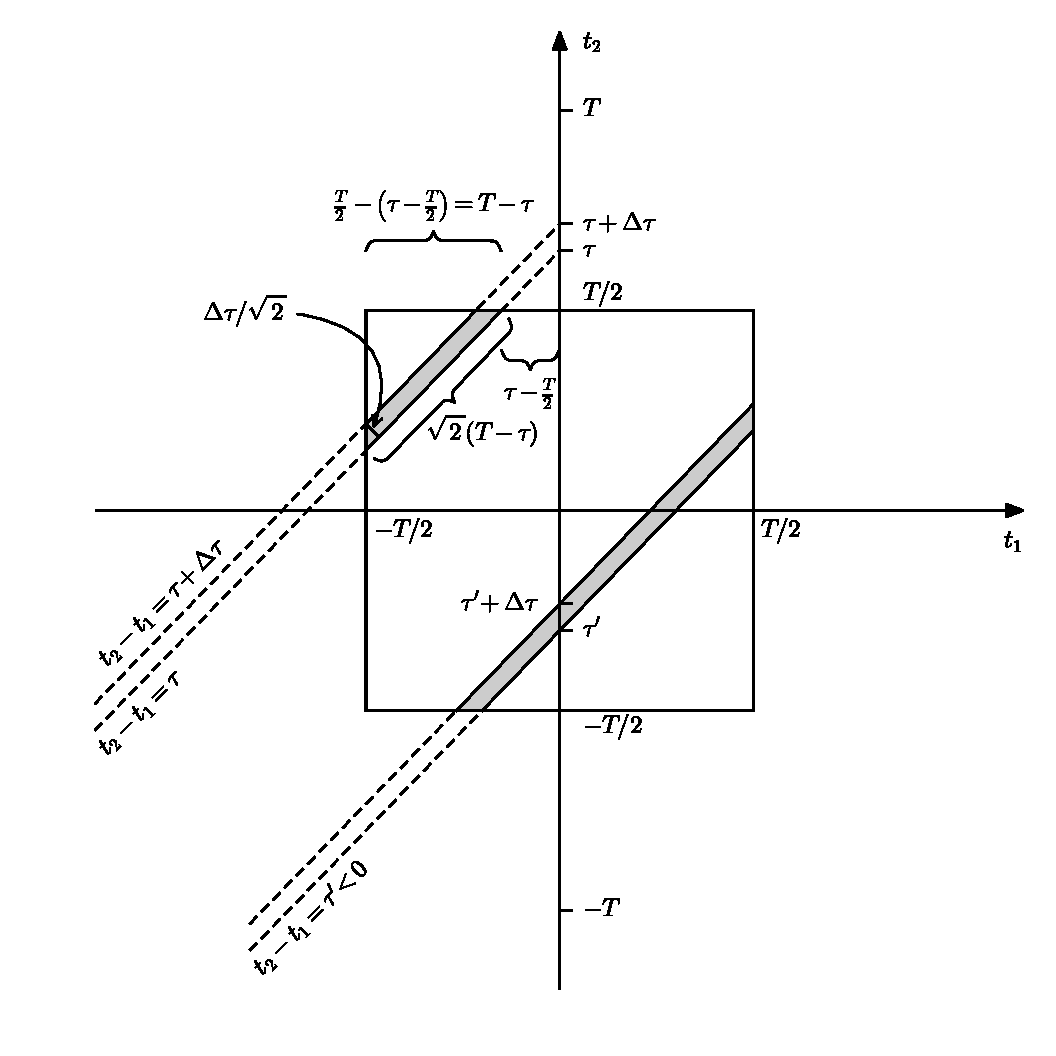
\includegraphics[width=0.9\columnwidth]{figuras/wiener_khintchine_integration_v2.eps}
\caption{\label{fig:wiener_khintchine_integration} Derivación del teorema de Wiener-Khintchine. En el plano \((t_1,\,t_2)\), el cuadrado es la región de integración de la ecuación \ref{eq:wiener_khintchine_integration}. En las regiones sombreadas, la función \(\varphi(t_2-t_1)\approx\varphi(\tau)\) es constante si \(\Delta\tau\to0\). La región sombreada en la parte superior corresponde a \(\tau>0\) y la inferior a \(\tau<0\). El área de la región para \(\tau>0\), que es un trapecio, es \((T-\tau)\Delta\tau-\Delta\tau^2/2\) y tiende a \((T-\tau)\Delta\tau\) con \(\Delta\tau\to0\).}
\end{center}
\end{figure}

La integral doble de la ecuación \ref{eq:wiener_khintchine_integration} puede convertirse en una integral simple observando que \(\varphi(t_2-t_1)\) es constante en cualquier recta \(t_2-t_1=\tau\) (con \(\tau\) fijo) en el plano \((t_1,\, t_2)\). Considérense dos de esas rectas, \(t_2-t_1=\tau\) y \(t_2-t_1=\tau+\Delta\tau\). Con \(\Delta\tau\to0\), la función \(\varphi(t_2-t_1)\approx\varphi(\tau)\) es constante sobre el área determinada por las rectas, región sombreada en la figura \ref{fig:wiener_khintchine_integration}. 
Dicha área es \((T-\tau)\Delta\tau\), y el volumen determinado por \(\varphi(t_2-t_1)\) sobre esa área es \(\varphi(\tau)(T-\tau)\Delta\tau\). Puede deducirse también que en el caso de  \(t_2-t_1=\tau'<0\), el volumen determinado por \(\varphi(t_2-t_1)\) sobre el área es \(\varphi(\tau')(T+\tau')\Delta\tau\). Por lo tanto, generalizando, el volumen sobre las regiones sombreadas en la figura \ref{fig:wiener_khintchine_integration} es \(\varphi(\tau)(T-|\tau|)\Delta\tau\). El volumen buscado sobre el área cuadrada en la figura, es la suma de los volúmenes sobre las todas franjas sombreadas que abarcan el cuadrado, y se obtiene integrando  \(\varphi(\tau)(T-|\tau|)\) en el rango significativo de \(\tau\), que es  \((-T,\,T)\), como se puede ver en la figura \ref{fig:wiener_khintchine_integration}. 
Por lo tanto,
\begin{align*}
  S_x&=\lim_{T\to\infty}\frac{1}{T}\int_{-T}^{T}\varphi(\tau)(T-|\tau|)\,d\tau\\
       &=\lim_{T\to\infty}\int_{-T}^{T}\varphi(\tau)\left(1-\frac{|\tau|}{T}\right)\,d\tau\\
       &=\int_{-\infty}^{\infty}\varphi(\tau)\,d\tau,
\end{align*}
donde en la última igualdad se asume que \(\int_{-\infty}^{\infty}|\tau|\varphi(\tau)\,d\tau\) es acotado, de forma que al dividir entre \(T\) y tomar el límite, el término tiende a cero. Sustituyendo la ecuación \ref{eq:wiener_khintchine_phi_def} en este resultado, se obtiene que
\[
  S_x(f) = \int_{-\infty}^{\infty}R_x(\tau)e^{-j2\pi f\tau}\,d\tau,
\]
concluyendo que la PSD de un proceso estacionario en sentido amplio es la transformada de Fourier de su función de autocorrelación,
\[
 R_x(\tau)\overset{\mathcal{F}}{\longleftrightarrow}S_x(f).
\]

La función de autocorrelación \(R_x(\tau)\) es una función simétrica conjugada, 
\[
 R_x(-\tau) = R^*_x(\tau),
\]
y la PSD \(S_x(f)\) es una función real (ver sección \ref{ap:fourier_transform_property_symmetry}). En el caso particular de procesos reales, tanto la autocorrelación como la PSD son funciones reales y pares.

El valor cuadrático medio \(\overline{|x(t)|^2}\) del proceso \(x(t)\) es la autocorrelación evaluada en cero,
\[
 R_x(0)=\overline{x^*(t)x(t)}=\overline{|x(t)|^2}=\overline{|x|^2},
\]
que se calcula como el promedio en el ensamble para cualquier valor de \(t\). En el caso de procesos estacionarios en sentido amplio, el resultado es independiente de \(t\). Además, la potencia promedio \(P_x\) del proceso aleatorio \(x(t)\) es su valor cuadrático medio \(\overline{|x|^2}\). Por el teorema de Wiener-Khintchine, se tiene que
\[
 R_x(\tau) = \int_{-\infty}^{\infty}S_x(f)e^{j2\pi f\tau}\,df.
\]
Por lo tanto,
\[
 P_x = \overline{|x|^2} =  R_x(0) = \int_{-\infty}^{\infty}S_x(f)\,df.
\]
Este resultado indica que la potencia \(P_x\) es la integral de la PSD \(S_x(f)\) en todas las frecuencias, justificando su definición como densidad espectral. El resultado es análogo al obtenido para señales determinísticas en la sección \ref{sec:psd_deterministic}.

\section{Aplicación: PSD de una señal PAM digital}\label{sec:pam_psd}

Una forma de transmitir mensajes digitales en banda base por un canal analógico es mediante la técnica denominada Modulación por Amplitud de Pulso (PAM, \emph{Pulse Amplitude Modulation}). Cada símbolo digital emitido por la fuente se codifica como un pulso analógico \(p(t)\) fijo modulado en amplitud según el valor del símbolo. Si el alfabeto de la fuente tiene \(M\) símbolos distintos (fuente \(M\)-ária), el pulso tomará \(M\) valores posibles de amplitud. La amplitud del pulso correspondiente al \(k\)-ésimo símbolo enviado es \(a_k\). La fuente emite un símbolo cada \(T_b\) segundos, por lo que la duración del pulso analógico \(p(t)\) es \(T_b\).

Teniendo en cuenta las consideraciones anteriores, la señal analógica transmitida, denominada señal PAM digital, es un tren de pulsos que se puede describir como
\begin{equation}\label{eq:digital_pam_process}
y(t)= \sum_{k=-\infty}^{\infty}a_kp(t-kT_b-\alpha),
\end{equation}
donde \(\alpha\) es el retardo del primer pulso (\(k=0\)). Como la secuencia de símbolos que emitirá la fuente es desconocida, las amplitudes \(a_k\) se modelan como variables aleatorias con características estadísticas que dependen de la fuente. También se asume desconocido el retardo \(\alpha\) del primer símbolo respecto al origen temporal, y se modela como una variable aleatoria que toma valores equiprobables en el intervalo \([0,\, T_b)\). Por lo tanto, \(y(t)\) es un proceso aleatorio. En la figura \ref{fig:digital_pam} se muestra el pulso \(p(t)\) y una realización de \(y(t)\).

\begin{figure}[!htb]
\begin{center}
\includegraphics[width=0.9\columnwidth]{figuras/digital_pam.eps}
\caption{\label{fig:digital_pam} Señal PAM digital.}
\end{center}
\end{figure}

El objetivo es calcular la PSD  del proceso \(y(t)\). La estrategia es calcular la función de autocorrelación \(R_y(\tau)\) de \(y(t)\) y aplicar la transformada de Fourier al resultado. Pero para  garantizar la existencia de la PSD, hay que verificar que el proceso es al menos estacionario en sentido amplio. Se comenzará estudiando si la media \(\overline{y(t)}\) es constante. Se asume la razonable hipótesis adicional de que las variables aleatorias \(a_k\) son independientes de la variable aleatoria \(\alpha\). Aplicando el operador esperanza en ambos lados de la igualdad en la ecuación \ref{eq:digital_pam_process},
\begin{align*}
 \overline{y(t)} &=  \overline{\sum_{k=-\infty}^{\infty}a_kp(t-kT_b-\alpha)}\\
   &\overset{(a)}{=}\sum_{k=-\infty}^{\infty}\overline{a_kp(t-kT_b-\alpha)}\\
   &\overset{(b)}{=}\sum_{k=-\infty}^{\infty}\overline{a_k}\overline{p(t-kT_b-\alpha)},
\end{align*}
donde en \((a)\) se aplicó la propiedad de linealidad de la esperanza y en \((b)\) se empleó que las variables aleatorias \(a_k\) y \(\alpha\) son independientes.

Asumiendo que la fuente es estacionaria y por lo tanto la estadística de los símbolos emitidos no cambia con el tiempo, la media de la amplitud \(\overline{a_k}\) es una constante independiente de \(k\) y por lo tanto,
\begin{equation}\label{eq:pam_psd_derivation_mean}
 \overline{y(t)} = \overline{a_k}\sum_{k=-\infty}^{\infty}\overline{p(t-kT_b-\alpha)}.
\end{equation}
Usando la definición de esperanza, el término dentro de la sumatoria puede escribirse como
\[
 \overline{p(t-kT_b-\alpha)} = \int_{-\infty}^{\infty}p(t-kT_b-\alpha)f(\alpha)\,d\alpha,
\]
donde \(f(\alpha)\) es la función densidad de probabilidad de la variable aleatoria \(\alpha\), que por ser uniforme en \([0,\,T_b)\), se tiene que
\begin{equation}\label{eq:pam_psd_derivation_alpha_pdf}
 f(\alpha)=
  \left\{\begin{array}{ll}
  1/T_b & 0 \leq t < T_b\\
  0 & \textrm{en otro caso}\\ \end{array} \right.,
\end{equation}
y entonces,
\begin{align*}
 \overline{p(t-kT_b-\alpha)} &= \frac{1}{T_b}\int_{0}^{T_b}p(t-kT_b-\alpha)\,d\alpha\\
  &\overset{(a)}{=}-\frac{1}{T_b}\int_{t-kT_b}^{t-(k+1)T_b}p(\beta)\,d\beta\\
  &\overset{(b)}{=}\frac{1}{T_b}\int_{t-(k+1)T_b}^{t-kT_b}p(\beta)\,d\beta,
\end{align*}
donde en \((a)\) se realizó el cambio de variable de integración \(\beta=t-kT_b-\alpha\) y en \((b)\) se intercambiaron los límites de integración. Sustituyendo el resultado en la ecuación \ref{eq:pam_psd_derivation_mean}, se tiene que la media del proceso \(y(t)\) es
\[
 \overline{y(t)} = \frac{\overline{a_k}}{T_b}\sum_{k=-\infty}^{\infty}\int_{t-(k+1)T_b}^{t-kT_b}p(\beta)\,d\beta.
\]
Notar que para un valor de \(t\) fijo, la expresión consiste en la suma de infinitas integrales en intervalos adyacentes de largo \(T_b\), que en conjunto abarcan todos los reales desde \(-\infty\) a \(\infty\). Por lo tanto,
\[
 \overline{y(t)}=\frac{\overline{a_k}}{T_b}\int_{-\infty}^{\infty}p(\beta)\,d\beta.
\]
De esta ecuación, se concluye que la media del proceso \(y(t)\) es una constante independiente del tiempo \(t\).

Si en el modelo no se hubiera incluido la variable aleatoria \(\alpha\), puede deducirse a partir de la ecuación \ref{eq:pam_psd_derivation_mean} que la media del proceso sería
\[
 \overline{y(t)} = \overline{a_k}\sum_{k=-\infty}^{\infty}p(t-kT_b).
\]
Por tratarse de una función periódica de período \(T_b\), el proceso no es estacionario, ni siquiera en sentido amplio. Los procesos cuya estadística cambia de forma periódica con el tiempo se llaman cicloestacionarios, y en general pueden convertirse en procesos estacionarios mediante la introducción de una variable aleatoria \(\alpha\) como en este ejemplo.

Luego de haber verificado que la media es constante, se procede a calcular la autocorrelación,
\begin{align*}
 R_y(\tau) &= \overline{y(t)}\overline{y(t+\tau)}\\
   &= \overline{\sum_{k=-\infty}^{\infty}a_kp(t-kT_b-\alpha)}\overline{\sum_{m=-\infty}^{\infty}a_mp(t+\tau-mT_b-\alpha)}\\
   &\overset{(a)}{=}\sum_{k=-\infty}^{\infty}\sum_{m=-\infty}^{\infty}\overline{a_ka_mp(t-kT_b-\alpha)p(t+\tau-mT_b-\alpha)}\\
   &\overset{(b)}{=}\sum_{k=-\infty}^{\infty}\sum_{m=-\infty}^{\infty}\overline{a_ka_m}\;\overline{p(t-kT_b-\alpha)p(t+\tau-mT_b-\alpha)},
\end{align*}
donde en \((a)\) se aplicó la propiedad de linealidad de la esperanza y en \((b)\) se tuvo en cuenta que \(a_k\) y \(a_m\) son independientes de \(\alpha\). Realizando el cambio de variable \(m=k+n\), se tiene que
\[
 R_y(\tau) =\sum_{k=-\infty}^{\infty}\sum_{n=-\infty}^{\infty}\overline{a_ka_{k+n}}\;\overline{p(t-kT_b-\alpha)p(t+\tau-[k+n]T_b-\alpha)}.
\]
El primer término dentro de la doble sumatoria es la correlación entre las variables aleatorias \(a_k\) y \(a_{k+n}\), que se denotará \(\mathcal{R}_n\). Se asume que la fuente emisora de símbolos es estacionaria, por lo que la correlación no depende de \(k\). El segundo término, por ser la media respecto a la variable aleatoria \(\alpha\), se puede expresar como la integral, como se hizo antes. Por lo tanto,
\begin{align*}
 R_y(\tau) &=\sum_{n=-\infty}^{\infty}\mathcal{R}_n\sum_{k=-\infty}^{\infty}\int_{-\infty}^{\infty}p(t-kT_b-\alpha)p(t+\tau-[k+n]T_b-\alpha)f(\alpha)d\alpha\\
   &\overset{(a)}{=}\sum_{n=-\infty}^{\infty}\mathcal{R}_n\sum_{k=-\infty}^{\infty}\frac{1}{T_b}\int_{0}^{T_b}p(t-kT_b-\alpha)p(t+\tau-[k+n]T_b-\alpha)d\alpha,
\end{align*}
donde en \((a)\) se utilizó la ecuación \ref{eq:pam_psd_derivation_alpha_pdf} para sustituir \(f(\alpha)\). Realizando el cambio de variable de integración \(\beta=t-kT_b-\alpha\), la expresión queda
\begin{align*}
 R_y(\tau) &=\frac{1}{T_b}\sum_{n=-\infty}^{\infty}\mathcal{R}_n\sum_{k=-\infty}^{\infty}\int_{t-(k+1)T_b}^{t-kT_b}p(\beta)p(\beta+\tau-nT_b)d\beta\\
  &\overset{(a)}{=}\frac{1}{T_b}\sum_{n=-\infty}^{\infty}\mathcal{R}_n\int_{-\infty}^{\infty}p(\beta)p(\beta+\tau-nT_b)d\beta,
\end{align*}
donde en \((a)\) se usó el mismo argumento que antes para combinar la sumatoria y la integral. Notando que la integral es la autocorrelación temporal (o determinística), definida en la ecuación \ref{eq:deterministic_autocorr_def}, de \(p(t)\) evaluada en \(\tau-nT_b\), se llega a que
\begin{equation}\label{eq:pam_autocorrelation}
 R_y(\tau) =\frac{1}{T_b}\sum_{n=-\infty}^{\infty}\mathcal{R}_n\psi_p(\tau-nT_b),
\end{equation}
con
\[
 \mathcal{R}_n=\overline{a_ka_{k+n}}\qquad\textrm{y}\qquad \psi_p(\tau)=\int_{-\infty}^{\infty}p(t)p(t+\tau)dt.
\]

Para calcular la PSD de \(y(t)\), se aplica la transformada de Fourier a la ecuación \ref{eq:pam_autocorrelation},
\begin{align*}
 S_y(f)&=\mathcal{F}\left[\frac{1}{T_b}\sum_{n=-\infty}^{\infty}\mathcal{R}_n\psi_p(\tau-nT_b)\right]\\
   &\overset{(a)}{=}\frac{1}{T_b}\sum_{n=-\infty}^{\infty}\mathcal{R}_n\mathcal{F}\left[\psi_p(\tau-nT_b)\right],
\end{align*}
donde en \((a)\) se aplicó la propiedad de linealidad de la transformada de Fourier. En la sección \ref{sec:autocorr_and_esd_relation} se vio que la autocorrelación y la densidad espectral de energía forman un par de transformadas de Fourier, es decir, si \(p(t)\overset{\mathcal{F}}{\longleftrightarrow}P(f)\), se cumple que 
\(\psi_p(\tau)\overset{\mathcal{F}}{\longleftrightarrow}|P(f)|^2\). Por lo tanto,
\[
 \mathcal{F}\left[\psi_p(\tau-nT_b)\right]=|P(f)|^2e^{-j2\pi fnT_b},
\]
en donde se usó además la propiedad de desplazamiento temporal de la transformada de Fourier (sección \ref{ap:fourier_transform_property_time_shift}). Por lo tanto, la PSD de la señal PAM digital queda
\begin{equation}\label{eq:pam_psd1}
  S_y(f)=\frac{|P(f)|^2}{T_b}\sum_{n=-\infty}^{\infty}\mathcal{R}_ne^{-j2\pi fnT_b}
\end{equation}

La expresión anterior es válida en el caso en que la secuencia de símbolos emitidos por la fuente es un proceso estacionario en sentido amplio. Se considera a continuación el caso particular en que los símbolos son independientes, con media \(\mu_a\) y varianza \(\sigma_a^2\). La correlación \(\mathcal{R}_n\) es entonces
\begin{align*}
\mathcal{R}_n&= \overline{a_ka_{k+n}}\\
&\overset{(a)}{=}\left\{ 
\begin{array}{l l}
\overline{a_k^2}, & k=0\\
\overline{a_k}\;.\;\overline{a_{k+n}}, & k\neq0 \end{array} \right.\\
&\overset{(b)}{=}\left\{ 
\begin{array}{l l}
\sigma_a^2+\mu_a^2, & k=0\\
\mu_a^2, & k\neq0, \end{array} \right.
\end{align*}
en donde en \((a)\) se usó que las variables aleatorias \(a_k\) y \(a_{k+n}\) son independientes y en \((b)\) que \(\sigma_a^2= \overline{(a_k-\mu_a)^2}=\overline{a^2_k}-\mu_a^2\) y por lo tanto, \(\overline{a^2_k}=\sigma_a^2+\mu_a^2\).
Sustituyendo este resultado en la ecuación \ref{eq:pam_psd1}, se tiene que
\[
S_y(f)=\frac{|P(f)|^2}{T_b}\left(\sigma_a^2+\mu_a^2\sum_{n=-\infty}^{\infty}e^{-j2\pi fnT_b}\right).
\]
Teniendo en cuenta la siguiente identidad matemática (ver apéndice \ref{ap:impulse_train_fourier_series})
\[
\sum_{n=-\infty}^{\infty}e^{-j2\pi fnT_b}=\frac{1}{T_b}\sum_{n=-\infty}^{\infty}\delta\left(f-\frac{n}{T_b}\right),
\]
la PSD se puede expresar como
\[
S_y(f)=\frac{|P(f)|^2}{T_b}\left(\sigma_a^2+\frac{\mu_a^2}{T_b}\sum_{n=-\infty}^{\infty}\delta\left(f-\frac{n}{T_b}\right)\right),
\]
y operando se obtiene que
\[
S_y(f)=\frac{\sigma_a^2|P(f)|^2}{T_b}+\left(\frac{\mu_a}{T_b}\right)^2\sum_{n=-\infty}^{\infty}\left|P\left(\frac{n}{T_b}\right)\right|^2\delta\left(f-\frac{n}{T_b}\right).
\]

\newpage

\appendix

\section{Transformada de Fourier}\label{ap:fourier_transform}

En este apéndice no se pretende profundizar en los conceptos vinculados a la transformada de Fourier. Solo se incluye la definición y algunas propiedades con el objetivo de mostrar la notación empleada en el documento.

\subsection{Definiciones}

La \textbf{transformada de Fourier} de una señal \(g(t)\) se define como
\begin{equation}\label{eq:fourier_transform_def}
 G(f)=\int_{-\infty}^{\infty}g(t)e^{-j2\pi ft}\,dt.
\end{equation}
Si la variable independiente \(t\) de la señal \(g(t)\) representa el tiempo en segundos (s), la variable \(f\) de la transformada \(G(f)\) representa frecuencia en Hertz (Hz). En ciertas condiciones, es posible determinar \(g(t)\) a partir de la transformada \(G(f)\) mediante la \textbf{transformada inversa de Fourier},
\begin{equation}\label{eq:inverse_fourier_transform_def}
 g(t)=\int_{-\infty}^{\infty}G(f)e^{j2\pi ft}\,df.
\end{equation}
Se dice que \(G(f)\) es la transformada directa de \(g(t)\) y \(g(t)\) es la transformada inversa o la antitransformada de \(G(f)\). Equivalentemente, se dice que \(g(t)\) y \(G(f)\) forman un par de transformadas de Fourier. Simbólicamente, se denota como
\[
 G(f)=\mathcal{F}\left[g(t)\right]\qquad \textrm{y} \qquad g(t)=\mathcal{F}^{-1}\left[G(f)\right]
\]
o
\[
g(t)\overset{\mathcal{F}}{\longleftrightarrow}G(f).
\]

Como se mencionó antes, el dominio de la transformada de Fourier es la frecuencia. De forma equivalente, el dominio de la transformada de Fourier puede representarse en frecuencia angular, definida como \(\omega = 2\pi f\) con unidades de radianes por segundo (rad/s). En ese caso, la transformada directa e inversa son
\[
 G(\omega)=\int_{-\infty}^{\infty}g(t)e^{-j\omega t}\,dt \qquad\textrm{y}\qquad g(t)=\frac{1}{2\pi}\int_{-\infty}^{\infty}G(\omega)e^{j\omega t}\,d\omega.
\]
Este resultado se obtiene directamente de aplicar el cambio de variable \(\omega = 2\pi f\) a la definición de la transformada de Fourier de las ecuaciones \ref{eq:fourier_transform_def} y \ref{eq:inverse_fourier_transform_def}.

\subsection{Algunas propiedades}

\subsubsection{Propiedades de simetría}\label{ap:fourier_transform_property_symmetry}

\begin{enumerate}[(i)]
 \item \textbf{Señal real}: la transformada de Fourier de una señal real es una función \textbf{simétrica conjugada} (función hermítica). Es decir, si \(G(f)\) es la transformada de Fourier de \(g(t)\), se cumple que,
 \[
  \textrm{si}\qquad
  \left\{\begin{array}{l}
  g(t)\textrm{ es una función real}\\
  \\
  G(f)=\mathcal{F}\left[g(t)\right] \end{array} \right.
  \qquad\Rightarrow\qquad G(-f)=G^*(f)
 \]
 Demostración: partiendo de la transformada de Fourier de la ecuación \ref{eq:fourier_transform_def} evaluada en \(-f\) y operando, se tiene que
 \begin{align*}
  G(-f)&=\int_{-\infty}^{\infty}g(t)e^{j2\pi ft}\,dt\\
    &\overset{(a)}{=}\left[\int_{-\infty}^{\infty}g^*(t)e^{-j2\pi ft}\,dt\right]^*\\
    &\overset{(b)}{=}\left[\int_{-\infty}^{\infty}g(t)e^{-j2\pi ft}\,dt\right]^*\\
    &\overset{(c)}{=}G^*(f),
 \end{align*}
donde en \((a)\) se conjugó dos veces manteniendo la igualdad y se empleó la propiedad de que el conjugado de la integral es la integral del argumento conjugado\footnote{Esta propiedad se cumple porque la variable de integración es real.} y que el conjugado del producto es el producto de los factores conjugados, en \((b)\) se tiene en cuenta que \(g(t)\) es real y por lo tanto, \(g(t)=g^*(t)\), y en \((c)\) se reconoce que la integral entre paréntesis es la transformada de Fourier de \(g(t)\).
\item \textbf{Señal simétrica conjugada}: la transformada de Fourier de una señal simétrica conjugada (hermítica) es \textbf{real}. Matemáticamente, se plantea como
\[
  \textrm{si}\qquad
  \left\{\begin{array}{l}
  g(t)=g^*(-t)\\
  \\
  G(f)=\mathcal{F}\left[g(t)\right] \end{array} \right.
  \qquad\Rightarrow\qquad G(f)=G^*(f)
 \]
 Demostración: partiendo de la transformada de Fourier y operando, se ve que
\begin{align*}
  G(f)&=\int_{-\infty}^{\infty}g(t)e^{-j2\pi ft}\,dt\\
    &\overset{(a)}{=}\int_{-\infty}^{\infty}g^*(-t)e^{-j2\pi ft}\,dt\\
    &\overset{(b)}{=}-\int_{\infty}^{-\infty}g^*(x)e^{j2\pi fx}\,dx\\
    &\overset{(c)}{=}\int_{-\infty}^{\infty}g^*(x)e^{j2\pi fx}\,dx\\
    &\overset{(d)}{=}\left[\int_{-\infty}^{\infty}g(x)e^{-j2\pi fx}\,dx\right]^*\\
    &\overset{(e)}{=}G^*(f),
 \end{align*}
 donde en \((a)\) se emplea la hipótesis de que \(g(t)\) es hermítica, es decir, se cumple que \(g(t)=g^*(-t)\), en \((b)\) se realizó el cambio de variable \(x=-t\), en \((c)\) se intercambiaron los límites de integración, en \((d)\) se conjuga la integral y el argumento, y en \((e)\) se reconoce que la integral entre paréntesis es la transformada de Fourier de \(g(t)\).
\item \textbf{Señal real y par}: la transformada de Fourier de una señal real y par es \textbf{real y par}.\\
Demostración: la propiedad es consecuencia de la combinación de las dos propiedades anteriores.
\end{enumerate}


\subsubsection{Propiedad de desplazamiento temporal}\label{ap:fourier_transform_property_time_shift}

La propiedad de desplazamiento temporal indica que
\[
 \textrm{si}\qquad g(t)\overset{\mathcal{F}}{\longleftrightarrow}G(f)\qquad\Rightarrow\qquad g(t-t_0)\overset{\mathcal{F}}{\longleftrightarrow}e^{-j2\pi ft_0}G(f)
\]
Demostración:
\begin{align*}
 \mathcal{F}\left[g(t-t_0)\right] &=\int_{-\infty}^{\infty}g(t-t_0)e^{-j2\pi ft}\,dt\\
   &\overset{(a)}{=}\int_{-\infty}^{\infty}g(x)e^{-j2\pi f(x+t_0)}\,dx\\
   &=e^{-j2\pi ft_0}\int_{-\infty}^{\infty}g(x)e^{-j2\pi fx}\,dx\\
   &\overset{(b)}{=}e^{-j2\pi ft_0}G(f),
\end{align*}
donde en \((a)\) se realizó el cambio de variable \(x=t-t_0\) y en \((b)\) se reconoce que la integral es la transformada de Fourier \(G(f)\) de \(g(t)\) (ecuación \ref{eq:fourier_transform_def}).

\section{Representación en series de Fourier de un tren de impulsos periódico}\label{ap:impulse_train_fourier_series}
 
Se quiere demostrar que se cumple la siguiente igualdad,
\begin{equation}\label{eq:impulse_train_fourier_series}
\sum_{n=-\infty}^{\infty}\delta(t-nT)=\frac{1}{T}\sum_{n=-\infty}^{\infty}e^{j\frac{2\pi}{T}nt}.
\end{equation}

Considérese el tren de pulsos periódico de período \(T\),
\[
 \operatorname{III}_T(t)=\sum_{n=-\infty}^{\infty}\delta(t-nT).
\]
Por ser una función periódica, admite una representación en series de Fourier,
\[
 \operatorname{III}_T(t)=\sum_{n=-\infty}^{\infty}c_ne^{j\frac{2\pi}{T} nt},
\]
con
\[
 c_n=\frac{1}{T}\int_{-T/2}^{T/2} \operatorname{III}_T(t)e^{-j\frac{2\pi}{T}nt}\,dt.
\]
Por lo tanto,
\begin{align*}
 c_n&=\frac{1}{T}\int_{-T/2}^{T/2}\left[\sum_{n=-\infty}^{\infty}\delta(t-nT)\right]e^{-j\frac{2\pi}{T}nt}\,dt\\
   &\overset{(a)}{=}\frac{1}{T}\int_{-T/2}^{T/2}\delta(t)e^{-j\frac{2\pi}{T}nt}\,dt\\
   &\overset{(b)}{=}\frac{1}{T}\int_{-T/2}^{T/2}\delta(t)\,dt\\
   &\overset{(c)}{=}\frac{1}{T},
\end{align*}
donde en \((a)\) se considera \(\operatorname{III}_T(t)\) solo en el intervalo de integración, \(\operatorname{III}_T(t)=\delta(t)\) en \([-T/2,\,T/2]\), en \((b)\) se aplicó que \(\delta(t)f(t)=\delta(t)f(0)\) y en \((c)\) que \(\int\delta(t)\,dt=1\) en cualquier intervalo de integración que contenga el 0.

Finalmente, la representación en series de Fourier queda
\[
 \operatorname{III}_T(t)=\frac{1}{T}\sum_{n=-\infty}^{\infty}e^{j\frac{2\pi}{T} nt},
\]
verificando la igualdad indicada en la ecuación \ref{eq:impulse_train_fourier_series}.
 
\section{Deducción alternativa de la PSD de una señal PAM digital}

En este apéndice se presenta una deducción alternativa de la PSD de una señal PAM digital siguiendo el enfoque  basado en el capítulo 11 del libro \cite{Carlson2009}. Como se explicó en la sección \ref{sec:pam_psd}, una señal PAM digital se expresa como (ecuación \ref{eq:digital_pam_process}),
\[
y(t)= \sum_{k=-\infty}^{\infty}a_kp(t-kT_b-\alpha),
\]
donde \(p(t)\) es el pulso conformador de duración \(T_b\), \(a_k\) es la amplitud correspondiente al símbolo \(k\)-ésimo y \(\alpha\) es un retardo que se modela como una variable aleatoria de distribución uniforme en el intervalo \([0,\, T_b)\).

Para calcular la PSD \(S_y(f)\) de \(y(t)\) se usará la definición, dada por la ecuación \ref{eq:psd_random_definition}
\[
 S_y(f)=\lim_{T\to\infty}\overline{\left[\frac{|Y_T(f)|^2}{T}\right]},
\]
 donde \(Y_T(f)\) es la transformada de Fourier del proceso truncado en el tiempo \(y_T(t)=y(t)\Pi(t/T)\). 
 Se considera el tiempo de truncamiento \(T\) de forma que \(y_T(t)\) contenga un número entero de pulsos \(p(t)\),
 \begin{equation}\label{eq:pam_psd_alt_derivation_yt}
  y_T(t)= \sum_{k=-K}^{K}a_kp(t-kT_b-\alpha).
 \end{equation}
 De esta forma, el tiempo de truncamiento es \(T=(2K+1)T_b\) y por lo que \(y_T(t)\) contiene \(2K+1\) pulsos. El primer paso es aplicar la transformada de Fourier a la ecuación \ref{eq:pam_psd_alt_derivation_yt}. Por la propiedad de desplazamiento temporal de la transformada de Fourier, se cumple que
 \[
  p(t)\overset{\mathcal{F}}{\longleftrightarrow}P(f)\qquad\Rightarrow\qquad p(t-kT_b-\alpha)\overset{\mathcal{F}}{\longleftrightarrow}P(f)e^{-j2\pi f(kT_b+\alpha)},
 \]
 por lo que
 \[
  Y_T(f)=P(f)\sum_{k=-K}^{K}a_ke^{-j2\pi f(kT_b+\alpha)}.
 \]
Luego,
\begin{align*}
 |Y_T(f)|^2&=Y_T(f)Y_T^*(f)\\
   &=|P(f)|^2\sum_{k=-K}^{K}a_ke^{-j2\pi f(kT_b+\alpha)}\sum_{m=-K}^{K}a_m^*e^{j2\pi f(mT_b+\alpha)}\\
   &=|P(f)|^2\sum_{k=-K}^{K}\sum_{m=-K}^{K}a_ka_m^*e^{-j2\pi f(k-m)T_b},
\end{align*}
y tomando la esperanza queda,
\begin{align*}
 \overline{|Y_T(f)|^2}&=\overline{|P(f)|^2\sum_{k=-K}^{K}\sum_{m=-K}^{K}a_ka_m^*e^{-j2\pi f(k-m)T_b}}\\
  &=|P(f)|^2\sum_{k=-K}^{K}\sum_{m=-K}^{K}\overline{a_ka_m^*}e^{-j2\pi f(k-m)T_b}.
\end{align*}
\(\overline{a_ka_m^*}\) es la correlación entre las variables aleatorias \(a_k\) y \(a_m\) y se denotará \(\mathcal{R}_{k,\,m}\). Teniendo en cuenta que la fuente es estacionaria, la correlación no depende de los instantes \(k\) y \(m\) específicos, si no de la diferencia \(k-m\), cumpliéndose que \(\mathcal{R}_{k,\,m}=\mathcal{R}_{k-m}\), por lo tanto,
 \[
  \overline{|Y_T(f)|^2}=|P(f)|^2\sum_{k=-K}^{K}\sum_{m=-K}^{K}\mathcal{R}_{k-m}e^{-j2\pi f(k-m)T_b}.
 \]
Definiendo la función \(\varphi_{k-m}\) como
\begin{equation}\label{eq:pam_psd_alt_derivation_phi}
  \varphi_{k-m}=\mathcal{R}_{k-m}e^{-j2\pi f(k-m)T_b},
\end{equation}
el resultado obtenido se puede escribir como
\begin{equation}\label{eq:pam_psd_alt_derivation_Y_t}
 \overline{|Y_T(f)|^2}=|P(f)|^2\sum_{k=-K}^{K}\sum_{m=-K}^{K}\varphi_{k-m} 
\end{equation}
\begin{figure}[!htb]
\begin{center}
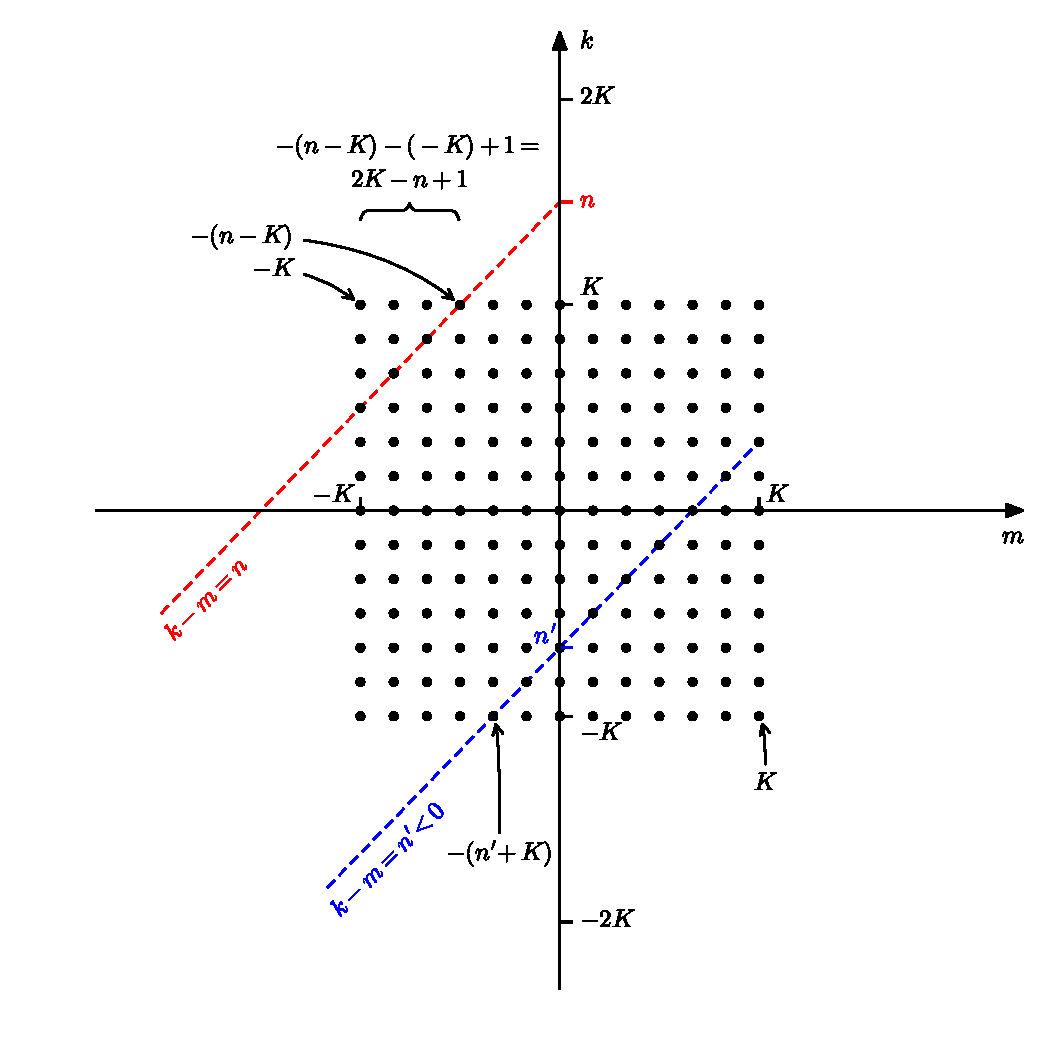
\includegraphics[width=0.9\columnwidth]{figuras/digital_pam_double_summation.eps}
\caption{\label{fig:digital_pam_double_summation}Derivación de la PSD de una señal PAM digital. En el plano  \((m,\,k)\), los puntos indican las coordenadas \(m\) y \(k\) de todos los sumandos \(\varphi_{k-m}\) de la doble sumatoria de la ecuación \ref{eq:pam_psd_alt_derivation_Y_t}. La doble sumatoria se puede expresar como una sumatoria simple teniendo en cuenta que \(\varphi_{k-m}\) es constante en cada diagonal \(k-m=n\), con \(n\) fijo. La recta en rojo indica una diagonal  \(k-m=n\) para \(n\) positivo, donde se puede ver que hay \(2K-n+1\) sumandos. Un caso con \(n\) negativo se muestra en la diagonal en azul, y contiene \(2K+n+1\) términos. Generalizando, en cada diagonal \(k-m=n\) hay \(2K-|n|+1\) sumandos.}
\end{center}
\end{figure}
La doble sumatoria de la  ecuación anterior consiste en la suma de los valores de \(\varphi_{k-m}\) para los valores de \(m\) y \(k\) en el cuadrado del plano  \((m,\,k)\) mostrado en la figura  \ref{fig:digital_pam_double_summation}. Esta doble sumatoria puede expresarse como una sumatoria simple notando que \(\varphi_{k-m}\) es constante en las diagonales \(k-m=n\) (con \(n\) fijo) en el plano \((m,\,k)\). Como se aprecia en la figura \ref{fig:digital_pam_double_summation}, en cada diagonal \(k-m=n\geq0\), hay  \(2K-n+1\) sumandos de valor \(\varphi_n\). También puede deducirse de la figura que en el caso en que \(n<0\), la cantidad de sumandos en la diagonal \(k-m=n\) es  \(2K+n+1\). Por lo tanto, generalizando, hay \(2K-|n|+1\) sumandos de valor \(\varphi_n\) en cada diagonal \(k-m=n\), con \(-2K\leq n\leq 2K\), y la doble sumatoria de la ecuación \ref{eq:pam_psd_alt_derivation_Y_t} se puede expresar como,
\begin{align*}
 \sum_{k=-K}^{K}\sum_{m=-K}^{K}\varphi_{k-m}&=\sum_{n=-2K}^{2K}(2K-|n|+1)\varphi_n\\
   &=(2K+1)\sum_{n=-2K}^{2K}\left(1-\frac{|n|}{2K+1}\right)\varphi_n.
\end{align*}
Sustituyendo este resultado y la ecuación \ref{eq:pam_psd_alt_derivation_phi} en la ecuación \ref{eq:pam_psd_alt_derivation_Y_t}, se llega a que
\[
 \overline{|Y_T(f)|^2}=|P(f)|^2(2K+1)\sum_{n=-2K}^{2K}\left(1-\frac{|n|}{2K+1}\right)\mathcal{R}_{n}e^{-j2\pi fnT_b},
\]
y la PSD se obtiene dividiendo entre \(T\) y tomando el límite \(T\to\infty\), como indica la ecuación \ref{eq:psd_random_definition}. Recordando que se había considerando \(T=(2K+1)T_b\) y tomando el límite \(K\to\infty\), la PSD es
\[
 S_y(f)=\lim_{K\to\infty}\frac{|P(f)|^2}{T_b}\sum_{n=-2K}^{2K}\left(1-\frac{|n|}{2K+1}\right)\mathcal{R}_{n}e^{-j2\pi fnT_b}.
\]
Asumiendo que \(\sum_{n=-\infty}^{\infty}|n|\mathcal{R}_n\) es acotado, se concluye que
\[
 S_y(f)=\frac{|P(f)|^2}{T_b}\sum_{n=-\infty}^{\infty}\mathcal{R}_{n}e^{-j2\pi fnT_b},
\]
coincidiendo con el resultado de la ecuación \ref{eq:pam_psd1}, que es lo que se quería demostrar.
 
\bibliographystyle{ieeetr}
\bibliography{signal_power_and_psd}

\end{document}
